\documentclass[]{report}
\usepackage[francais]{babel}
\usepackage[utf8]{inputenc}
\usepackage{graphicx} %'affichage des images

\title{Rapport projet conception logicielle}
\author{Romuald GAFFE\and Yanis COSNEFROY\and Vy Vu NGUYEN PHUONG\and Alexandre BOURGOIN}
\date{\today}


\begin{document}
\maketitle 
\tableofcontents
\part{Objectifs du projet}
\section{Présentation du concept}
Tout d'abord, nous avons choisi de créer un puzzle block puisque nous avions plus d'affinité et d'idées en rapport avec ce sujet. Nous voulions que ce jeu soit simple d'utilisation afin que tout le monde puisse y jouer. Le jeu que nous avons développé est composé de 4 modes de jeux, le premier étant le mode de jeu solo, il se présente sous forme d'une grille carré de 10 cases de côté. Le joueur obtient 3 pièces à placer sur la grille tirées aléatoirement parmi un total de 30 pièces(toutes orientations inclus). Les pièces qui apparaissent doivent toutes être placés dans la grille avant que les suivantes soit tirés. Si le tirage courant du joueur ne peut pas être placé alors un écran de fin de jeu s'affiche, montrant le score de la personne. Sur ce menu, le joueur aura la possibilité de retourner au menu principal ou de recommencer une partie. Ensuite le jeu se compose d'un mode multijoueur. Le premier étant contre une intelligence artificielle ayant le même mode de fonctionnement que le mode solo. Seul le score actuel de l'intelligence artificielle figure sur l'écran du joueur afin d'éviter d'en copier la stratégie. Le second mode multijoueur est, lui, un mode joueur contre joueur en local sur une même machine. Les grilles des joueurs s'affichent l'une après l'autre afin de limiter, de même, l'imitation de la stratégie adverse. Le dernier mode de jeu est un mode joueur contre joueur également mais en ligne où le but est de faire le plus de points.

\section{Cahier des charges}


\section{Exemples du jeux publiés}
Voici plusieurs block-puzzle provenant de jeux.fr, et des applications pour android: \\
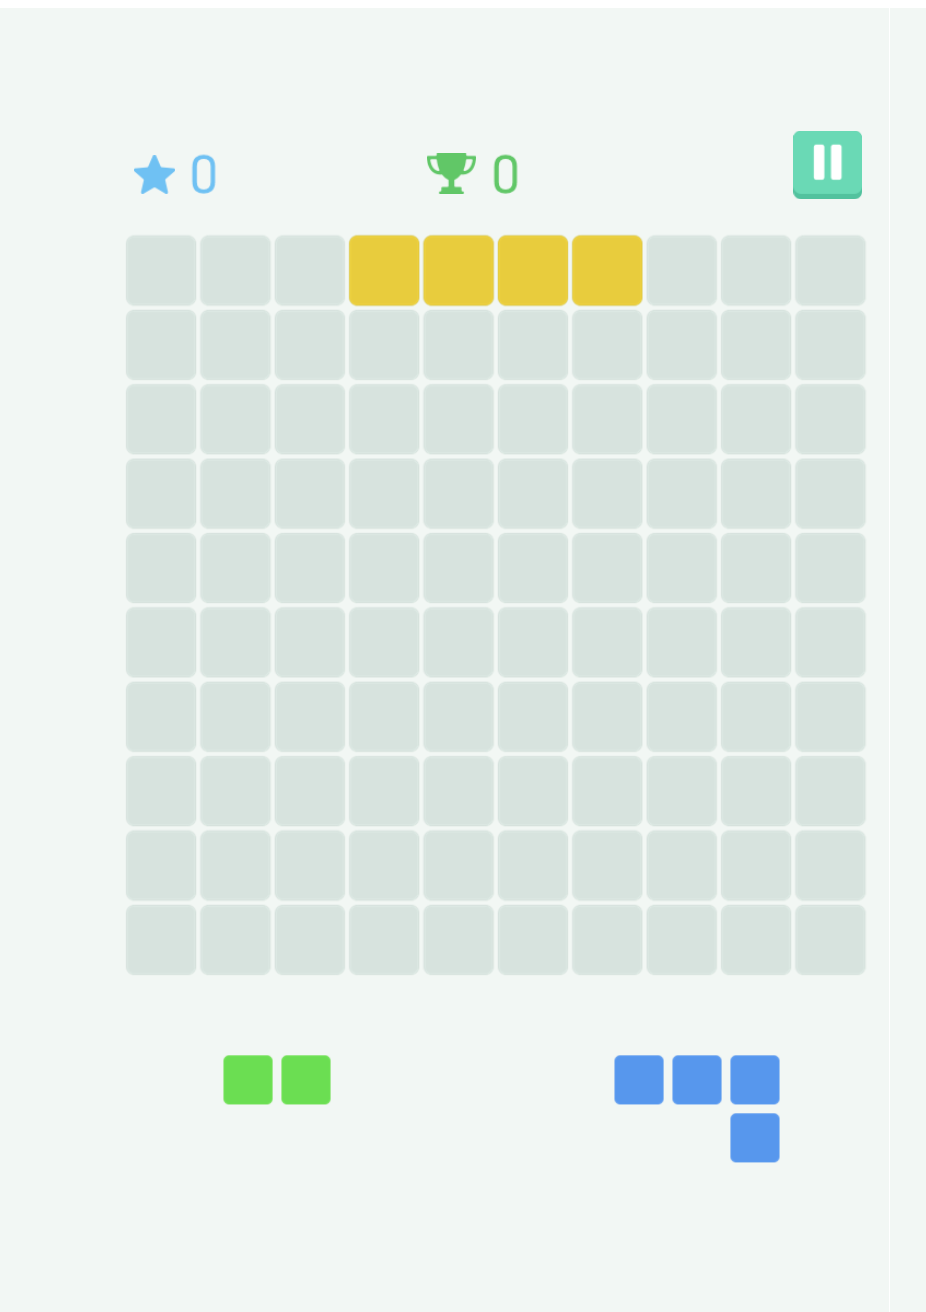
\includegraphics[scale=0.3]{images/jeuxPublie1.png}
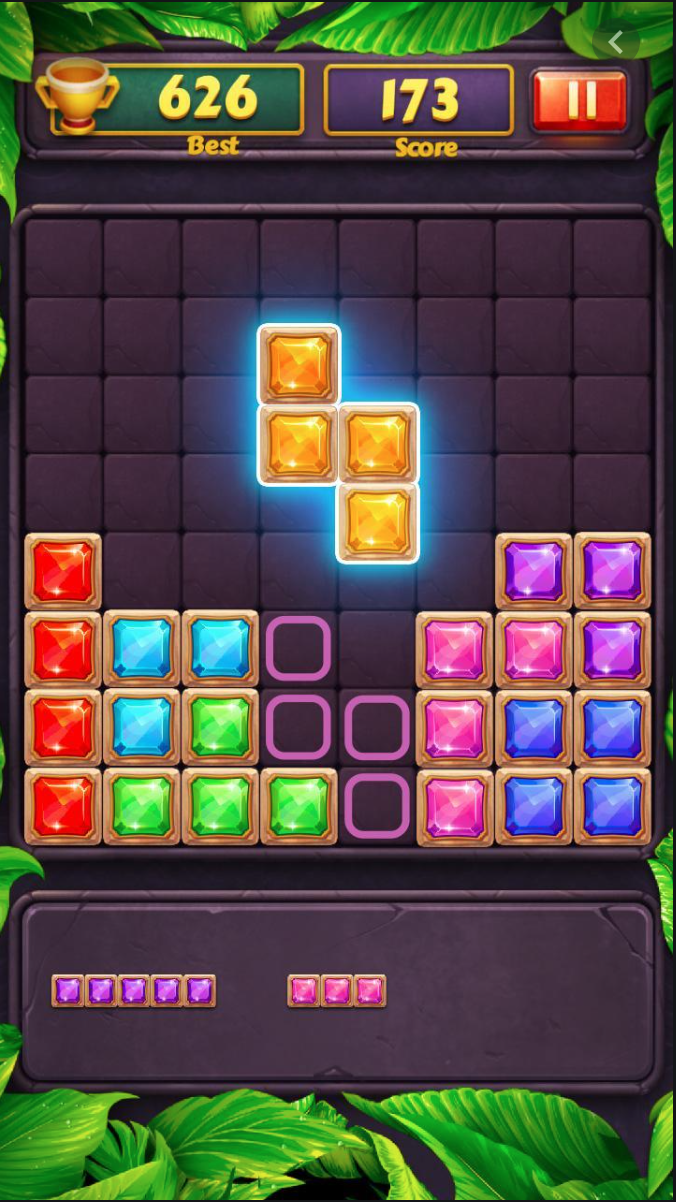
\includegraphics[scale=0.3]{images/jeuxPublie2.png}
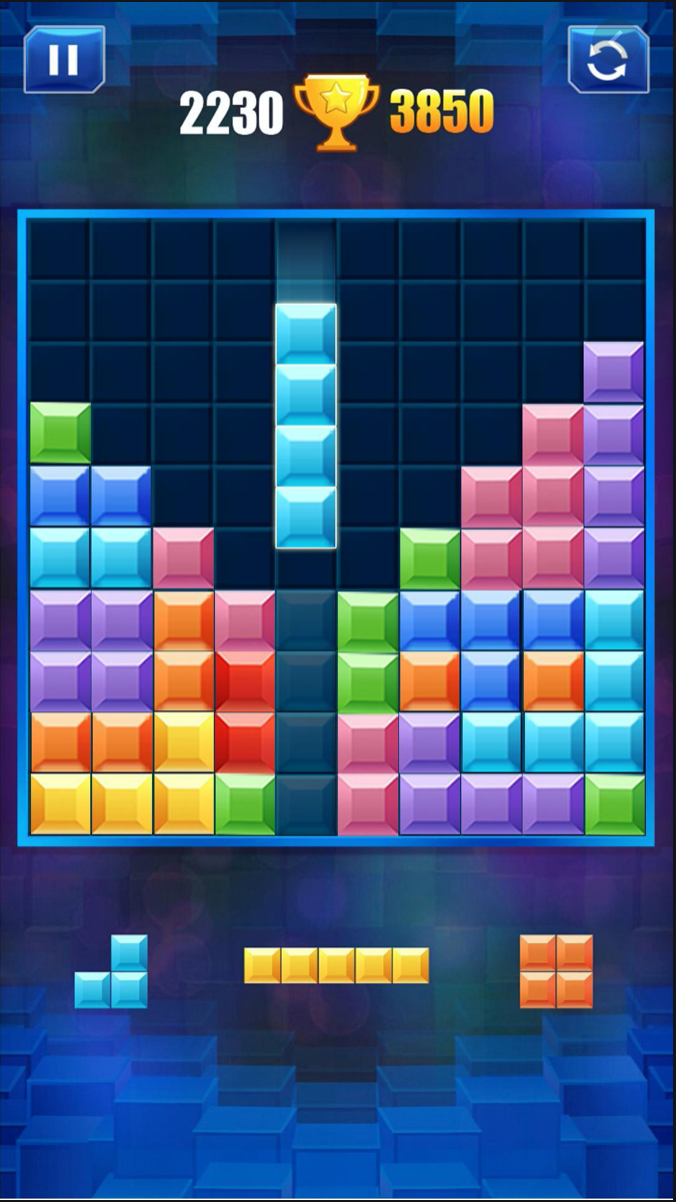
\includegraphics[scale=0.3]{images/jeuxPublie3.png}\\

On peut y retrouver les mêmes caractéristiques que notre projet. Notre projet a été conçu sur une base classique de block-puzzle qui réunit ces trois images montrées précédemment. Les différences entres ces block-puzzles et le nôtre sont l'aspect graphique ainsi que la sauvegarde du meilleur score établis sur le jeu par le joueur. On peut constater à l'essai de notre block-puzzle uniquement l'apparition des scores qui vont être actifs en fonction du jeu du joueur. Cependant nos règles sont un peu différentes par rapport au jeu déjà publié. On a décidé de ne pas rajouter de bonus ou d'aide à chaque fois qu'une ligne ou une colonne est remplie. C'est un choix volontaire pour provoquer une augmentation de concurrence de jeu avec d'autres joueurs mais aussi pour une adaptation plus développée de la difficulté de jeu. 
\part{Fonctionnalités implémentés}
\section{Mode solo}
\section{Mode multijoueur}
\subsection{Joueur vs Intelligence artificielle}
\subsection{Joueur vs Joueur en local}
\subsection{Joueur vs Joueur en ligne}

\part{Éléments techniques}
\section{La grille}
La grille est mise sous la forme d'une classe, 
\section{Les pièces}
\section{L'aléatoire}
\section{L'intelligence artificielle}
\section{Le réseau}

\part{Architecture du projet}
\section{Diagrammes des modules et des classes}
\section{Cas d'utilisation}

\part{Conclusion}


\end{document}
